\chapter{引言}
\label{chap1}
\fontsize{12bp}{14.4pt}

高能物理的主流理论框架是粒子物理标准模型,这是经过狄拉克、温伯格、费曼、朝永振一郎、汤川秀树等伟大物理学家一步步搭建起来,人类迄今为止最精确最普适用的理论模型,是物理学界的不朽杰作。但是,它仍然有很多不足之处,例如:没有把引力相互作用统一进来,无法解释暗物质之谜,无法完全解释宇宙中为什么正物质比反物质多那么多$\cdots\cdots$,这些都是留待我们新一代物理学者去攻克的问题。而实验是理论的基础,高能物理实验,也就成了人类突破未知的前哨站,其中最具有代表性的是欧洲大型强子对撞机(LHC)上的一系列粒子对撞实验,紧凑缪子螺线管(CMS)实验便是其中最大的实验之一。

最近两年先后出现了$\mu$子磁矩g-2实验结果与标准模型异常偏差\cite{muong-2},弱相互作用传播子W玻色子质量超出标准模型预言\cite{Wmass}等显著冲击标准模型的实验结果,极大地震惊和鼓舞了高能物理学界乃至整个科学界对新物理的期待。

同时,大型强子对撞机的CMS实验一方面对$\mu$子探测比其他实验有极大的优势,而且尚未完成大型强子对撞机第二轮运转时的对W质量的数据分析测量,这两点都为潜在的突破性发现提供了极佳条件。

作者参与了LHC上的CMS实验组,瞄准“上帝粒子”希格斯粒子的WW衰变过程,开发了CMS实验上首个对H$\to$WW喷注的多分类标记器,同时也可以用于X$to$WW共振态的搜寻,有助于实现对大动量希格斯粒子的精确测量,同时搜寻可能存在的新物理迹象。

\section{标准模型}
标准模型是当前粒子物理学(也称作高能物理)中得到广泛认可的理论框架,主要包括两方面的内容:第一,给出了构成我们大千世界的基本粒子,包括组成物质的费米子和负责传递各种相互作用的玻色子;第二,它统一了四种基本相互作用中的三种:电磁相互作用、弱相互作用和强相互作用,其中电磁相互作用和弱相互作用在标准模型中通过电弱统一理论进行描述,强相互作用通过量子色动力学进行描述。并且预言了赋予基本粒子质量的希格斯机制和希格斯粒子(也叫“上帝粒子”)。

标准模型的建立是在整个 20世纪下半叶,通过世界各地许多科学家的工作分阶段发展起来的,并且在 1970 年代中期的夸克存在实验后逐渐确定整个框架。从那时起,陶子\cite{Discovery_of_Tauon}(1975)、顶夸克\cite{top_quark_discovery}(1995)和希格斯玻色子\cite{Higgs_discovery}(2012)的发现进一步证明了标准模型的正确性。此外,标准模型也非常准确地预测了弱中性电流以及W 和 Z 玻色子的各种特性。
\subsection{标准模型的粒子组成}
\begin{figure}[H]
 \centering
 \caption{标准模型框架下的基本粒子}
 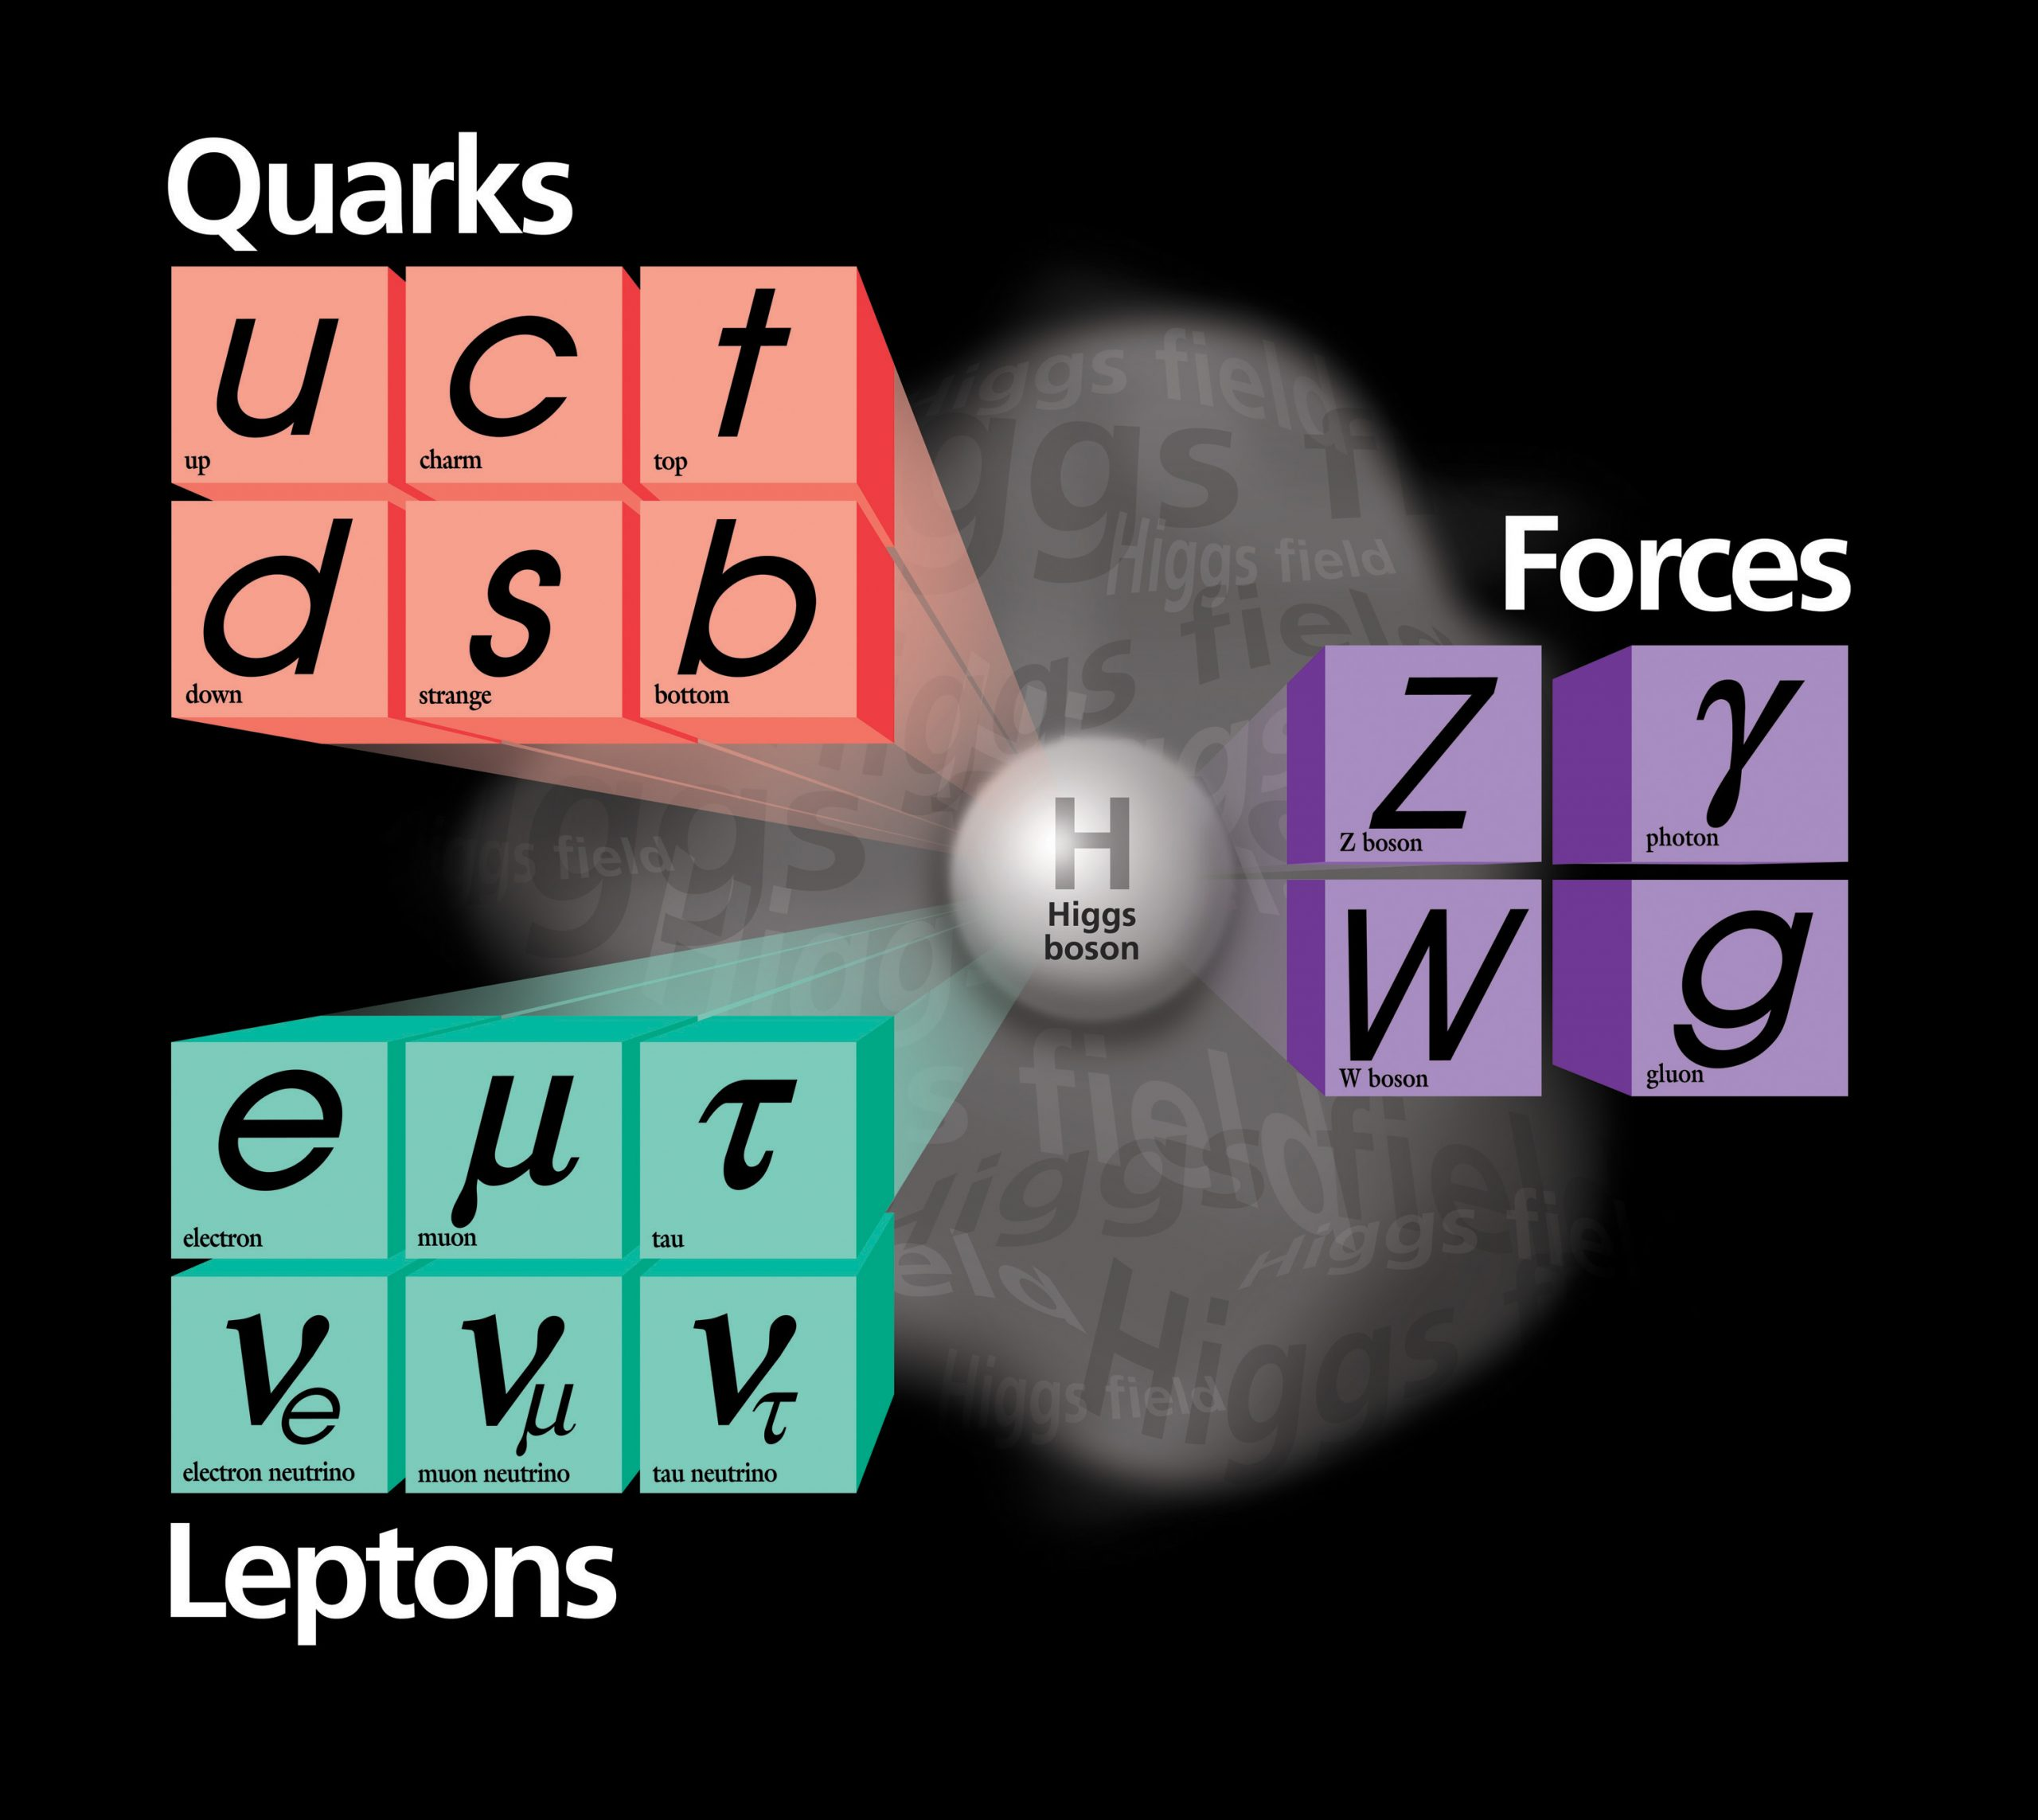
\includegraphics[height=10cm, width=10cm]{pictures/SM.jpg}
 \label{fig:1.1}
\end{figure}

标准模型共有61种基本粒子(见\textbf{表\ref{table:1.1}}),包含费米子及玻色子——费米子为拥有半奇数的自旋并遵守泡利不相容原理的粒子;玻色子则拥有整数自旋并且不遵守泡利不相容原理。简单来说,费米子就是组成物质的粒子而玻色子则负责传递各种作用力。

基本粒子中所有费米子自旋都为$\frac{1}{2}$,包括三代夸克及其反粒子,三代轻子及其反粒子,正反粒子具有相同的质量和相反的电荷。基本粒子中W,Z,光子传播电弱相互作用,自旋都为1;胶子传播强相互作用,自旋也为1;希格斯粒子自旋为0,通过Yukawa相互作用与粒子耦合并赋予它们质量。

值得一提的是,所有下型轻子(也就是中微子,包括电子中微子$\nu_e$,缪子中微子$\nu_\mu$,陶子中微子$\nu_\tau$)电荷为0且无色荷,所以不能参与电磁相互作用和强相互作用,只能参与难以直接探测的弱相互作用,只能通过量能器的能量沉积得到击中信息,并且很多时候根本探测不到,所以在实验中也经常被称为“消失的中性粒子”。
\begin{table}[htbp]
    \caption{基本粒子}\label{table:1.1}
    \centering
    \begin{tabular}{>{\centering\arraybackslash}p{1.5cm}%
    >{\centering\arraybackslash}p{2cm}%
    >{\centering\arraybackslash}p{2cm}%
    >{\centering\arraybackslash}p{1.5cm}%
    >{\centering\arraybackslash}p{2cm}%
    >{\centering\arraybackslash}p{2cm}%
    >{\centering\arraybackslash}p{1.5cm}}
    \toprule\toprule
    \textbf{名称} & \textbf{自旋类型} & \textbf{同位旋数(上下型)} & \textbf{世代数} & \textbf{电荷种类(正反粒子)} & \textbf{色荷种类} & \textbf{总计}\\
    \midrule
    夸克 & 半整数 & 2 & 3 & 2 & 3 & 36\\
    轻子 & 半整数 & 2 & 3 & 2 & \diagbox[height=0.6\line] & 12\\
    胶子 & 整数 & 1 & 1 & 1 & 8 & 8\\
    W & 整数 & 1 & 1 & 2 & \diagbox[height=0.6\line] & 2\\
    Z & 整数 & 1 & 1 & 1 & \diagbox[height=0.6\line] & 1\\
    光子 & 整数 & 1 & 1 & 1 & \diagbox[height=0.6\line] & 1\\
    希格斯 & 整数 & 1 & 1 & 1 & \diagbox[height=0.6\line] & 1\\
    \midrule
    总计 & & & & & & 61\\
    \bottomrule\bottomrule
\end{tabular}
\end{table}


\subsection{标准模型的相互作用}
\subsubsection{强相互作用}
强相互作用由$SU(3)_c$群的量子色动力学(QCD)描述,该群的生成元是8个线性无关矩阵$T^a=\frac{\lambda^a}{2}$,其中$\lambda^a$是Gell-Mann矩阵,a表示着8个色自由度,为了保证规范不变性,需要引入协变微分
\begin{equation}
    \left( D_\mu \right)_{ij} = \partial_\mu \delta_{ij} - i g \left( T_a \right)_{ij} \mathcal{A}^a_\mu,
\end{equation}
然后将拉氏量改写为
\begin{equation}
    \mathscr{L}_\mathrm{QCD} = \bar{\psi}_i  \left( i \gamma^\mu (D_\mu)_{ij} - m\, \delta_{ij}\right) \psi_j - \frac{1}{4}G^a_{\mu \nu} G^{\mu \nu}_a,
\end{equation}
这里的G表示为规范不变胶子场强度张量
\begin{equation}
    G^a_{\mu \nu} = \partial_\mu \mathcal{A}^a_\nu - \partial_\nu \mathcal{A}^a_\mu + g f^{abc} \mathcal{A}^b_\mu \mathcal{A}^c_\nu,
\end{equation}
其中${\mathcal {A}}_{\mu }^{a}(x)$是胶子场。

根据量子场论的规则和相关的费曼图,上述理论产生了三种基本相互作用:一个夸克可以发射(或吸收)一个胶子,一个胶子可以发射(或吸收)一个胶子,以及两个胶子可以直接互动。这与QED形成对比,在 QED 中只发生第一种相互作用,因为光子没有电荷。

使用上述拉氏量的详细计算表明,介子中夸克与其反夸克之间的有效势包含一项与夸克和反夸克之间的距离成比例增加的项($\propto r$ ),它表示粒子与其反粒子在远距离相互作用的某种“刚度”,类似于橡皮筋的熵弹性。这导致夸克被限制在强子内部,即介子和核子,具有特征半径$R_c\sim\SI{1}{fm}(=10^{-15}\si{m})$。

在一对正反夸克体系的能标(距离尺度)下,它们之间的强相互作用势能可以用如下式子表示
\begin{equation}
    V(r)=-\frac{4\alpha_S(r)}{3r}+kr,
\end{equation}
这里$\alpha_S(r)$是QCD耦合常数,是距离r(亦即能标)的函数,会随着能量的增大(距离的减小)而减小,这也被叫做\textbf{“渐近自由”}。

当距离增加时,势能也会随之增加,同时产生吸引力,所以我们看到正反夸克对不可能无限远离(因为势能不可能无限大),而往往被束缚在有限的距离内,这种现象就被称为\textbf{“夸克禁闭”}。同样的,当出现单个夸克时,我们可以认为这就相当于正反夸克无限远离,所以粒子物理实验中是不会有夸克单独射出,而是会从夸克海中生成新的正反夸克对与单夸克结合形成束缚态,从而降低单夸克的强相互作用势能,这个过程中还往往伴随着强子化过程形成喷注(高能粒子束流)。


\subsubsection{电弱相互作用}
在粒子物理学中,电弱相互作用是电磁相互作用与弱相互作用的统一描述,而这两种作用都属于自然界中四种已知基本相互作用。在粒子物理的[GeV]及以下能标中,电磁作用与弱作用存在很大的差异,然而在能标超过W的不变质量,即至少在100[GeV]的能标下,这两种作用力会统一成的电弱相互作用。

数学上是用一个SU(2)$\otimes$U(1)的规范群统一描述电磁作用及弱作用。当中对应的零质量规范玻色子分别是三个来自SU(2)弱同位旋的W玻色子($W^+$、$W_0$和$W^−$)以及一个来自U(1)弱超荷的$B_0$玻色子。

在标准模型里$W^±$和$Z_0$玻色子和光子是经由$SU(2)\otimes U(1)_Y$的电弱对称性自发对称破缺成$U(1)_{em}$所产生的,此一过程称作希格斯机制(见希格斯玻色子)。$U(1)_Y$和$U(1)_{em}$都属于$U(1)$群,但两者不同;$U(1)_{em}$的生成元是电荷$Q=Y/2+T^3$,而其中Y是$U(1)_Y$(叫弱超荷)的生成元,$T^3$(弱同位旋的一个分量)则是$SU(2)$的其中一个生成元。

属于$SU(2)\otimes U(1)_Y$自由费米子场的拉氏量如下
\begin{equation}
    \mathscr{L}=i\Bar{\psi}\gamma^\mu\partial_\mu \psi
\end{equation}

对于场在$SU(2)\otimes U(1)_Y$的规范变换
\begin{equation}
    \psi \to\psi^\prime=e^{igT^a\Lambda^a(x)}e^{\frac{i}{2}g^\prime Y\zeta(x)}\psi,
\end{equation}
为了满足场在$SU(2)\otimes U(1)_Y$规范变换下的局域不变性,我们必须得引入协变微商$\mathcal{D}_\mu$以代替$\partial_\mu$:
\begin{equation}
    \mathcal{D}_\mu=\partial_\mu -igT^aW_\mu^a-i\frac{g^\prime}{2} Y B_\mu,
\end{equation}
其中$g$为$SU(2)_L$作用的耦合常数,$g^\prime$为$U(1)_Y$作用的耦合常数,$\displaystyle T^a=\frac{\sigma^a}{2}$是同位旋算符($\sigma^a$是泡利矩阵),$a$是欧式指标可取1,2,3(度量矩阵为3阶单位阵),$\mu$、$\nu$是四维指标。(这里也可以看出关系式$\displaystyle Q=T^3+\frac{Y}{2}$,粒子电荷等于同位旋第三分量加上超荷一半)

从而将带电弱相互作用的费米子场拉氏量改写为
\begin{equation}
    \mathscr{L}=i\Bar{\Psi}\gamma^\mu\mathcal{D}_\mu \Psi-\frac{1}{4}W^{\mu\nu}_a W^a_{\mu\nu}-\frac{1}{4}B^{\mu\nu}B_{\mu\nu},
\end{equation}
其中有三个带电的无质量玻色子$W^1,W^2,W^3$和一个无质量的中性玻色子B,由于对称性自发破缺,将会出现我们实验中观测到的有质量正负W玻色子,可表示为
\begin{equation}
    W^{\pm}=\frac{1}{\sqrt{2}}(W^1\mp iW^2)
\end{equation}

相应地,Z和$\gamma$光子可表示为
\begin{equation}
    \begin{pmatrix}
\gamma \\
Z \end{pmatrix} = \begin{pmatrix}
\cos \theta_\text{W} & \sin \theta_\text{W} \\
-\sin \theta_\text{W} & \cos \theta_\text{W} \end{pmatrix} \begin{pmatrix}
B \\
W_3 \end{pmatrix},
\end{equation}
其中$\theta_W$是电弱混合角,也被称为温伯格角。

\subsubsection{引入质量耦合的Higgs机制}
上面提到电弱统一中本来是无质量的$W^1,W^2$可通过自发对称破缺变为有质量的$W^\pm$,这就是通过希格斯机制实现的质量赋予。

因为电弱统一是$SU(2)\otimes U(1)$理论,讨论起来较为复杂,所以我们从U(1)群的希格斯机制开始讨论。

因为我们知道自旋为0质量为m的粒子的拉氏量为
\begin{equation}
    \mathscr{L}=(\partial_{\alpha} \phi)^*(\partial^{\alpha} \phi)-m^2\phi^*\phi -V(\phi^*\phi),
\end{equation}
反过来,如果一个拉氏量中有$\phi$的二阶项,那么它的系数就可以认为是场对应粒子的不变质量。

现在让我们考虑一个无质量标量场$\phi$,并将该场的拉氏量写为
\begin{equation}\label{eq:1.1}
    \mathscr{L}=\partial_{\mu}\bar{\phi}\partial^{\mu} \phi+\mu^2\bar{\phi}\phi -\lambda(\bar{\phi}\phi)^2,
\end{equation}
其中$\lambda$,$\mu$都大于0,希格斯势为$V=\lambda\bar{\psi}\psi)^2-\mu^2\bar{\psi}\psi$,该拉氏量满足$U(1)$的局域对称变换。显然这个类二次函数的最低值在$\bar{\phi}\phi\frac{|v|^2}{2}=\frac{-\mu^2}{2\lambda}$处(其中$v=\frac{\mu}{\sqrt{\lambda}}$也就是量子场论中的真空态),在$\phi$二维复平面上考虑$V$的高度就可以形成一个旋转对称墨西哥草帽的形状。

我们现在将原始的$\phi$写成$\phi=\phi_1+i\phi_2=(\varphi_1+v+i\varphi_2)/\sqrt{2}$,其中$v=\frac{\mu}{\sqrt{\lambda}}$当成真空态,$(\varphi_1+i\varphi_2)/\sqrt{2}$才当成我们现在要考虑的$U(1)$相互作用的粒子,我们知道$U(1)$相互作用的协变微分可以写为$\mathcal{D}_\mu=\partial_{\mu}+iqA_{\mu}$,把以上结果代入$U(1)$相互作用的拉氏量有
\begin{equation}
\begin{aligned}\mathscr{L} & =\frac{1}{2}[(\partial_{\alpha}+iqA_{\alpha})(\varphi_1+v+i\varphi_2)]^*
[(\partial^{\alpha}+iqA^{\alpha})(\varphi_1+v+i\varphi_2)]
-\ \frac{1}{4}F_{\alpha\beta}F^{\alpha\beta} \\
 & \qquad+\frac{\mu^2}{2}(\varphi_1+v+i\varphi_2)^*(\varphi_1+v+i\varphi_2)
-\ \frac{\lambda}{4}[(\varphi_1+v+i\varphi_2)^*(\varphi_1+v+i\varphi_2)]^2 ,\\
\end{aligned}
\end{equation}
化简后有
\begin{equation}
    \mathscr{L}=\frac{1}{2}(\partial_{\alpha}\varphi_1)(\partial^{\alpha}\varphi_1)
-\mu^2\varphi_1^2+\ \frac{1}{2}(\partial_{\alpha}\varphi_2)(\partial^{\alpha}\varphi_2)-\ \frac{1}{4}F_{\alpha\beta}F^{\alpha\beta} +\ \frac{1}{2}q^2 v^2 A_{\alpha}A^{\alpha}+ \mathscr{L}_{int}
\end{equation}

又因为$U(1)$对称性要求拉氏量在$\phi\to e^{i\theta(x)}\phi$旋转变换下不变,于是我们在局域变换中设定相位$\theta=-\arctan{(\phi_2/\phi_1)}$,并令$\phi\to \phi'=e^{i\theta}\phi=(\phi_1\cos{\theta}-\phi_2\sin{\theta})
+i(\phi_1\sin{\theta}+\phi_2\cos{\theta})$即可得到
\begin{equation}
    \mathscr{L}=\ \frac{1}{2} (\partial_{\alpha}\varphi_1)(\partial^{\alpha}\varphi_1) 
-\mu^2\varphi_1^2  -\ \frac{1}{4}F_{\alpha\beta}F^{\alpha\beta} +\ \frac{1}{2}q^2 v^2 A_{\alpha}A^{\alpha} +\mathscr{L}_{int},
\end{equation}
其中$F_{\alpha\beta}=\partial_\alpha A_\beta-\partial_\beta A_\alpha$

现在我们得到,$\varphi_1$是赋予质量的希格斯粒子场,其质量为$\sqrt{2}\mu$,$U(1)$规范矢量场$A_\alpha$的质量为$|q|\mu/\sqrt{\lambda}$,为对应规范玻色子的质量。

对于$SU(2)\otimes U(1)$群,希格斯场从$\varphi_1$变为了复值的
\begin{equation}
    \phi (x) ={\left ( \begin{matrix} \phi_1 + \mathrm{i} \phi_2\\ \phi_3 + \mathrm{i} \phi_4 \end{matrix} \right )},
\end{equation}
通过对称性自发破缺,产生了三个带质量的玻色子$W^\pm,Z$和一个无质量玻色子$\gamma$。

\section{超出标准模型的迹象}
\subsection{b夸克衰变中的轻子普适性异常}
在标准模型中,三代带电轻子都具有相同的电弱相互作用耦合强度,这也是轻子风味普适性(LFU)的一个显著特征。但是,轻子风味普适性(LFU)只是标准模型(SM)中特有的一种对称性,这在超出标准模型的理论中可能不成立。

在过去的几年,LHC上的LHCb实验合作组探测了一些以味道改变中性流(FCNC)作为传播子的稀有衰变过程\cite{LFU_violation},在这样的过程中来自标准模型的贡献会被压低,以此探测轻子风味普适性可能出现的异常从而搜寻超出标准模型的物理。2021年3月公布的结果\cite{LFU_violation}表明,来自LHCb的结果与之前来自其他b夸克工厂的实验结果,都暗示了可能的的超出标准模型迹象。

在测量实验中,研究人员们测量了B介子的衰变到$\mu$
子与衰变到电子的截面之比,为了简化,定义为$R_K$
\begin{equation}
    R_K\equiv BR(B^+\to K^+\mu^+\mu^-)/BR(B^+\to K^)
\end{equation}
这里$B^+$的价夸克是$u\bar{b}$,$K^+$的价夸克是$u\bar{s}$,所以这个过程本质上是$b\to s\ell^+\ell^-$。在这样的过程上检验轻子风味异常的好处有:充分压低标准模型贡献,同时能精确检验理论预测。在轻子风味普适性的假设下,$R_K$理论预言为$R_K^{th}=0.997\pm 0.011$,因此$R_K$的测量结果与1的任何显著偏离都意味着有超出标准模型的物理。

LHCb实验的挑战在于,虽然电子和$\mu$子以相同的方式参与弱电相互作用,但电子小得多的质量意味着它与探测器材料的相互作用比$\mu$子多得多。例如,电子在穿LHCb探测器时会辐射出大量的轫致辐射光子,与$\mu$子相比,这会降低电子的重建效率和信号分辨率。处理这种效应的关键是通过$J/\Psi\to e^+e^-$和$J/\Psi\to \mu^+\mu^-$衰变过程(已知它们具有相同的衰变概率)可用于校准和测试电子重建效率。同时,$J/\Psi$的高精度测试与轻子味道普适性兼容,这为实验分析提供了有力的交叉检验。在这次对$R_K$的更高精度与更大统计量测量中,LHCb合作组发现了更大显著度的轻子风味异常。
\begin{figure}[H]
 \centering
 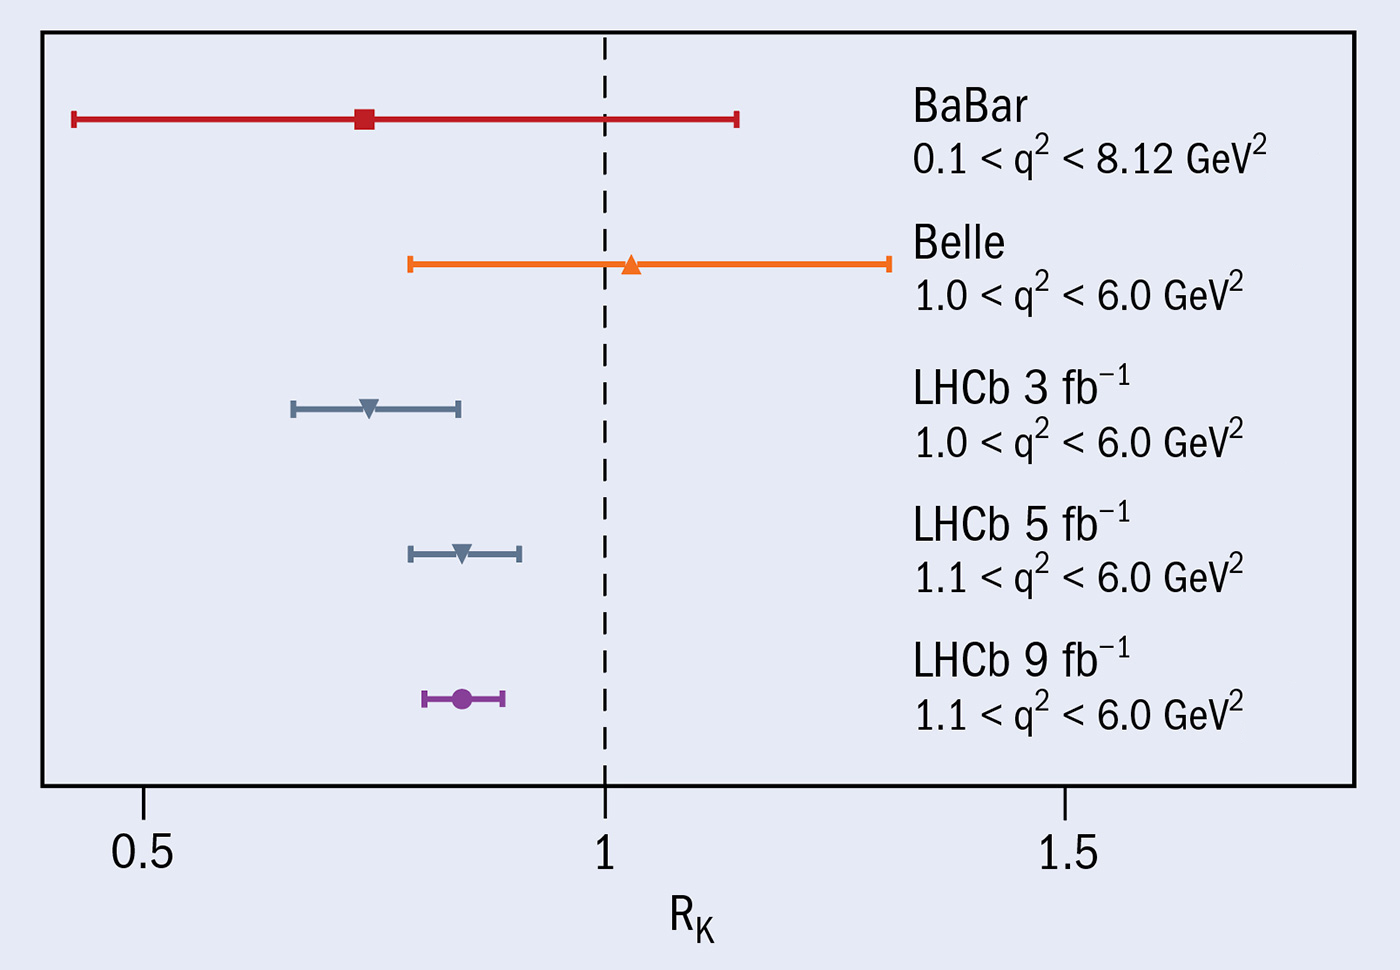
\includegraphics[height=10cm, width=14cm]{pictures/R_K_comparison.jpeg}
  \caption{$R_K$测量结果的比较\cite{RK_comparison_fig}:除了LHCb的结果,还展示了BaBar和Belle合作组的$B^+\to K^+\ell^+\ell^-$和$B^0\to K_S^0\ell^+\ell^-$测量的联合结果}
 \label{fig:1.2}
\end{figure}

此前LHCb分别在2019年\cite{RK_2019}和2017\cite{RKstar_2017}年对$R_K$和$R_K^*$(基于$B^0\to K^*\ell^+\ell^–$衰变过程)的测量已经显示了偏离1的迹象。而在这次对$R_K$的最新分析使用了大型强子对撞机(LHC)运行周期RUN 1和RUN 2 阶段中收集的完整数据。由于数据集增加了一倍,因此这次与之前的测量相比,精度有了显著提高(如\textbf{图\ref{fig:1.2}}所示),测量得到的$R_K$比率与 标准模型预测的偏离三个标准差(如\textbf{图\ref{fig:1.2}}所示)。这是第一次在任何单个B介子衰变中看到轻子风味普适性的异常高于3$\sigma$,对应测量值为$R_K=0.846^{+0.042}_{-0.039}(\text{stat.})^{+0.013}_{-0.012}(\text{ sys.})$。

LHCb 实验很好地阐明了这些衰变中可能存在的新物理。现在一系列使用完整Run 1 和 Run 2 数据集的与$b\to s\ell^+\ell^-$相关测量正在进行中。在LHC第二次长时间关闭期间,对探测器的重大升级将在Run 3及以后的阶段提供测量精度上一个阶跃式的变化。

尽管现阶段下结论还为时过早,但轻子风味普适性的这种偏差与过去十年中在$b\to s\ell^+\ell^-$和类似过程中表现出来的异常模式是一致的。特别是,这个被数据加强的$R_K$异常可以与这个衰变过程中的其他测量结果(包括角不对称性和衰减率)一起用来作为支持新物理的证据。这些都等待未来进一步的分析。

\subsection{$\mu$子g-2实验结果与标准模型的偏差}
$\mu$子是一种类似于电子的基本粒子,和电子一样带有一个单位负电荷、自旋为1/2,但具有更大的质量,$\mu$子的质量大约是电子的200倍。$\mu$子与同属于轻子的电子和$\tau$子具有相似的性质,人们至今未发现轻子具有任何内部结构。

像电子一样,$\mu$子的行为就好像它们有一个微小的内部磁铁。在强磁场中,$\mu$子磁铁的方向会进动或摆动,就像陀螺或陀螺仪的轴一样。内部磁铁的强度决定了 $\mu$ 子在外部磁场中进动的速率,我们用称为“g因子”的参数表示这块“磁铁”的强度和旋转速度。这个数字可以用量子场论进行超高精度计算。对于标准模型中的费米子,普适的g的物理定义是
\begin{equation}
    \boldsymbol \mu = g {e \over 2m} \mathbf S 
\end{equation}
其中e是单位电荷大小,m是基本粒子不变质量,$\mathbf S $是自旋,$\boldsymbol\mu$是磁矩。按照狄拉克方程的计算,基本费米子的g=2。

根据量子场论的计算(由于真空态和量子涨落),对于$\mu$子,g的值略大于 2,我们主要关心g和2的差异,因此得名“g-2”实验。这种与2的差异是由量子场论的高阶贡献引起的。在高精度测量g-2并将其值与理论预测进行比较时,物理学家将发现实验是否与理论相符。任何超过误差允许的偏差都会暗示着自然界中存在尚未发现的亚原子粒子。

2021年,美国费米国家实验室的 Muon g-2实验备受期待的首个结果表明\cite{muong-2},在前所未有的精确度测量下,$\mu$子的g因子与标准模型计算结果存在较大偏差。几十年来,g-2的实验和理论差异就已经被测量过,这个里程碑式的结果,更是进一步确认了这个差异。
\begin{figure}[H]
 \centering
 \caption{g因子的标准模型理论值与实验的偏差\cite{muong-2_fig}}
 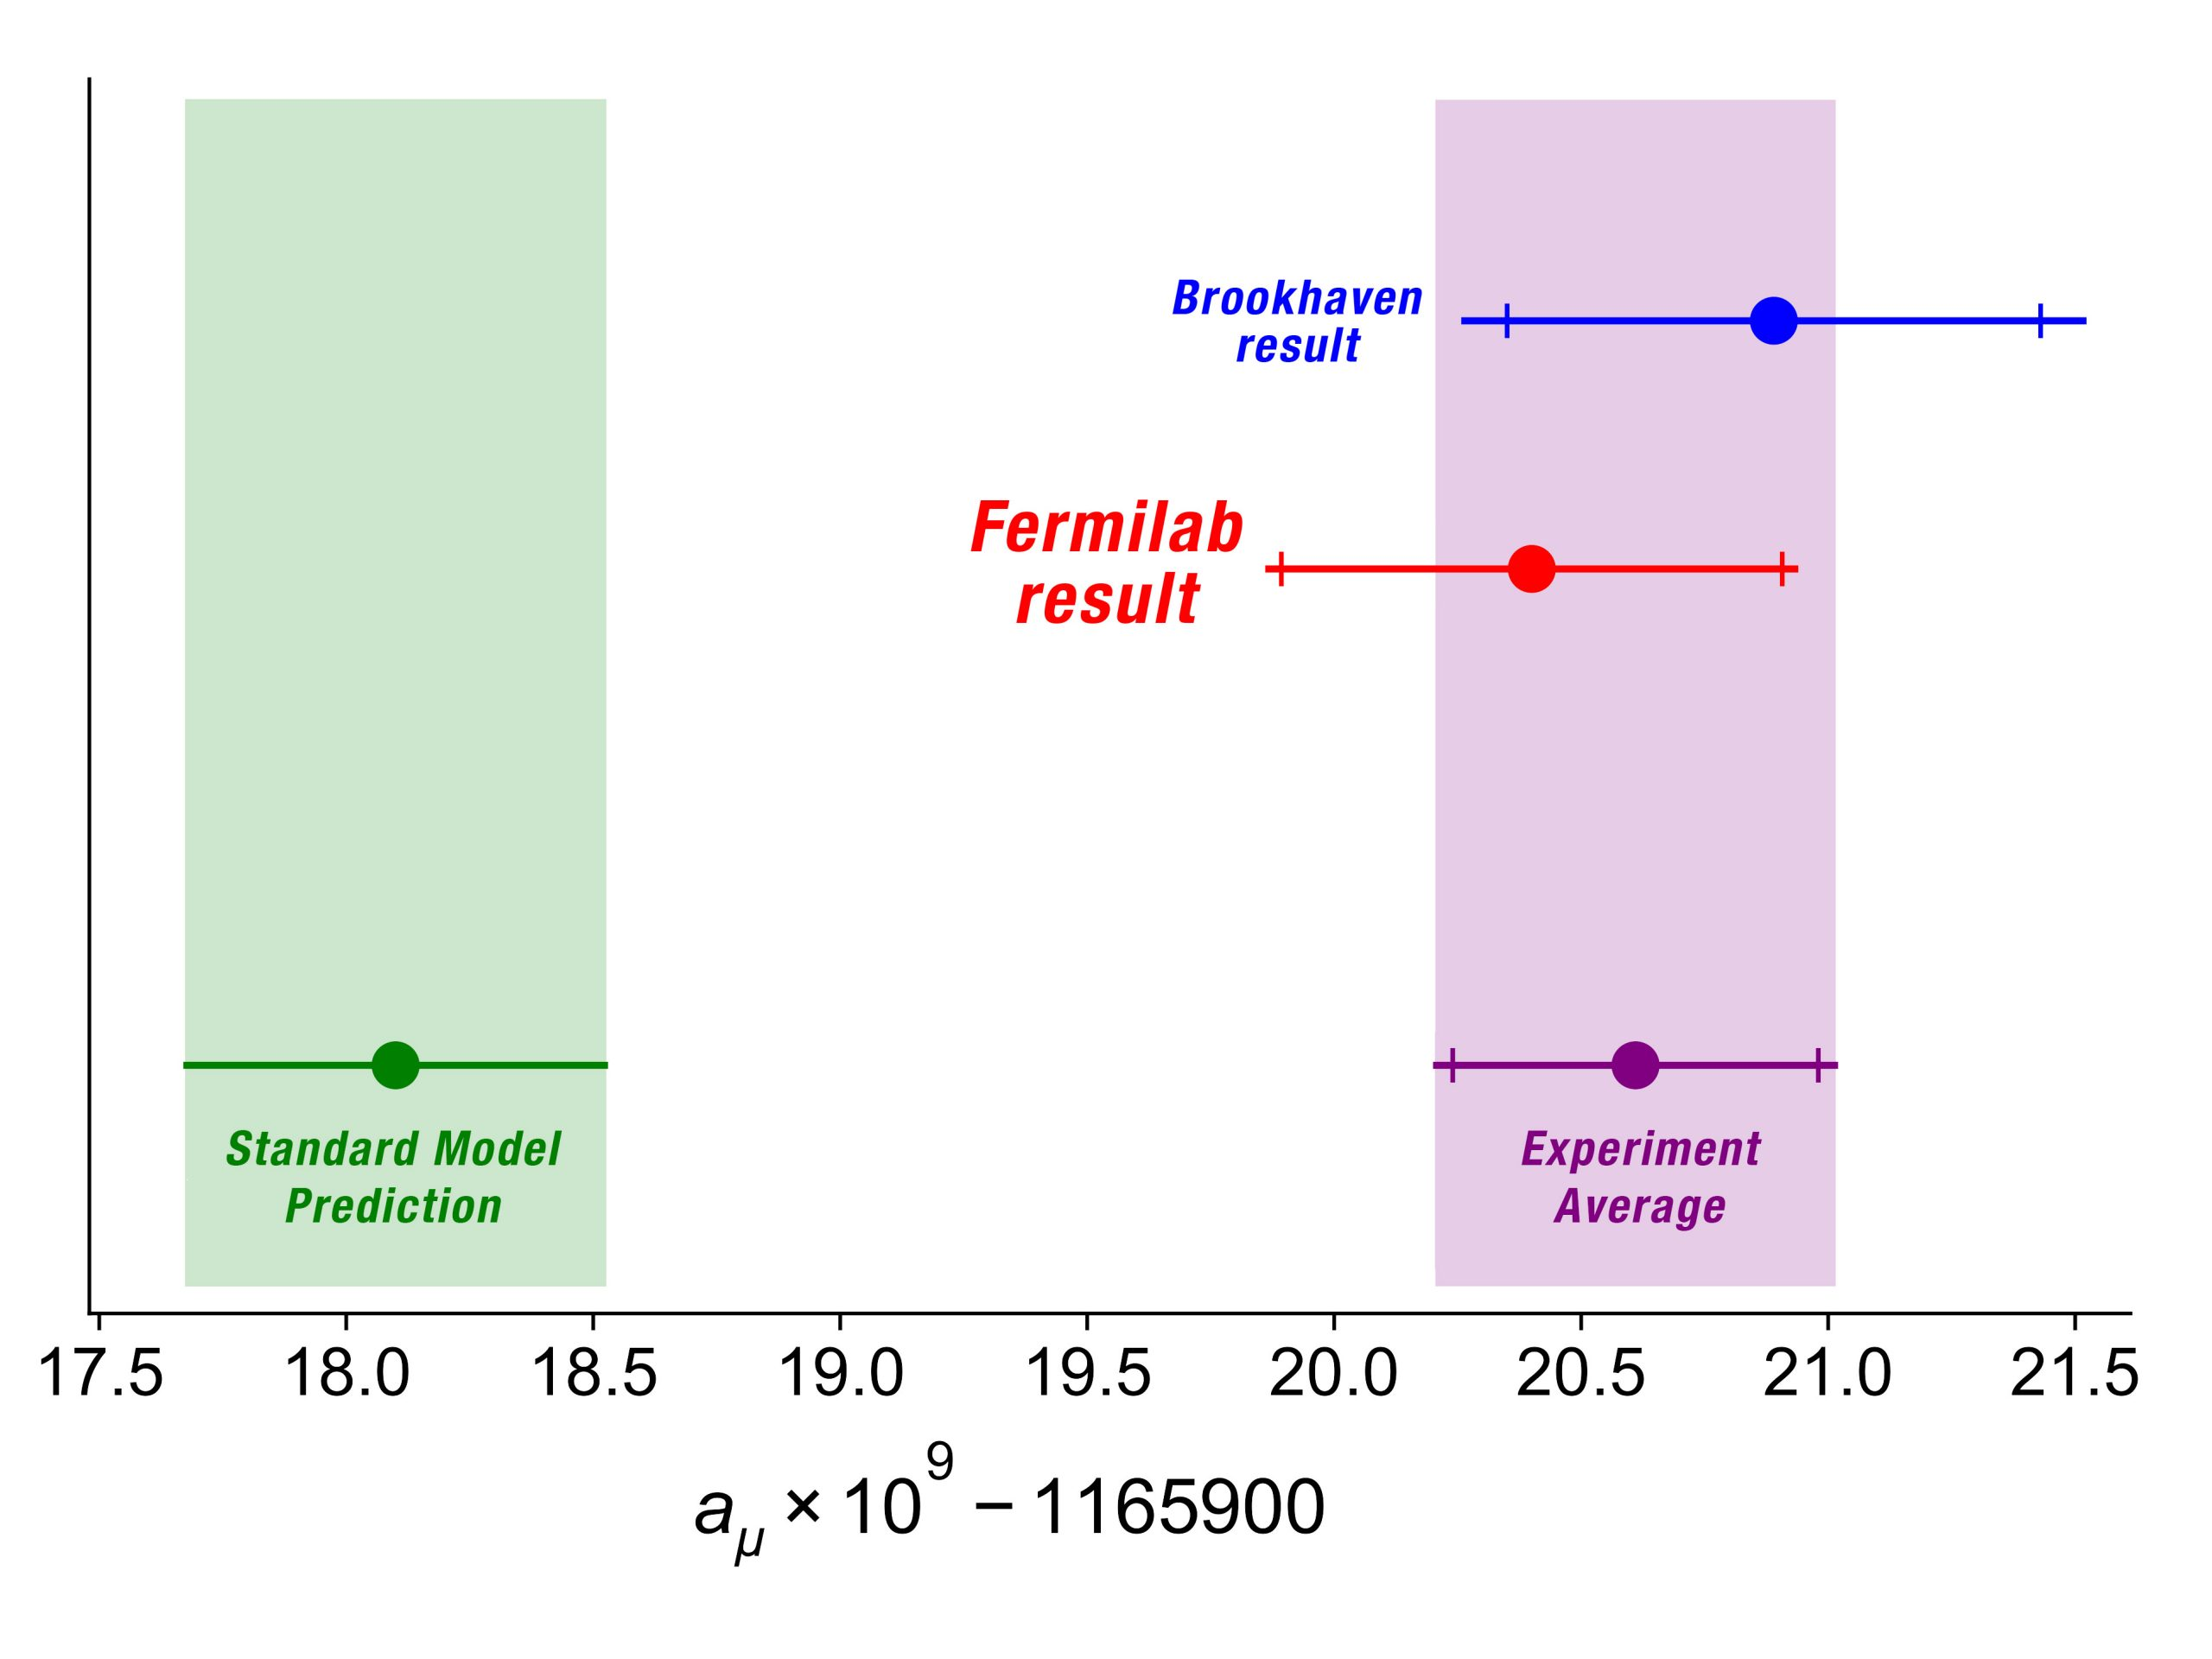
\includegraphics[height=10cm, width=12cm]{pictures/Muon-g-2-results-plot.jpeg}
 \label{fig:1.3}
\end{figure}

当 $\mu$子在费米实验室的Muon\ g-2磁铁中绕圈旋转时,它们同时会与与量子涨落不断生成或湮灭的亚原子粒子相互作用。与这些短寿命粒子的相互作用会影响g因子的值,导致$\mu$子非常轻微的进动加速或减速。标准模型极其精确地预测了这种所谓的异常磁矩。但是,如果量子涨落中包含标准模型未考虑的额外相互作用力或粒子,那将进一步影响$\mu$子的g因子大小。

公认的$\mu$子g因子理论值为:g=2.00233183620(86)。而费米实验室的Muon\ g-2 实验宣布的新实验结果为:g=2.00233184122(82)。(见上\textbf{图\ref{fig:1.3}})

费米实验室和布鲁克海文的联合结果显示,实验测量与理论的差异显著度为$4.2\sigma$(标准偏差),尽管略低于公认具有说服力的新物理证据所需的$5\sigma$阈,但$4.2\sigma$表明这次与标准模型的冲突结果是统计涨落的可能性约为四万分之一。

在运行的第一年,即2018年,费米实验室收集的数据就比之前所有$\mu$子g因子实验的总和还要多。目前已完成对第一次运行中超过80亿个$\mu$子的运动的分析。正在进行第二次和第三次实验的数据分析,第四次正在进行中,第五次正在计划中。到目前为止,只分析了不到6\%的实验最终将收集的数据。结合所有五次运行的结果,$\mu$子的g因子将得到更加精确地测量,从而更确定地揭示新物理是否隐藏在量子涨落中。

\subsection{超重的W玻色子}
W玻色子是弱相互作用的媒介粒子。它参与太阳发光和粒子衰变的反应过程。标准模型给出的W质量理论计算值为$M_W=(80357\pm6)$MeV。该值基于复杂的标准模型计算,通过将 W 玻色子的质量与另外两个粒子的质量的测量联系起来:顶夸克(于1995 年在费米实验室的Tevatron对撞机中发现\cite{top_quark_discovery}),希格斯玻色子(2012年在欧洲核子研究中心的大型强子对撞机上发现\cite{Higgs_discovery})。

过去40年来,许多对撞机实验都对W玻色子质量进行了测量,这些测量都是具有挑战性和十分复杂的。在2022年4月公布的美国费米国家实验室的W质量测量则\cite{Wmass}达到了更高的精度——经过10年的仔细分析和审查,美国能源部费米国家加速器实验室的科学家宣布,他们已经实现了迄今为止对W玻色子质量的最精确测量。

\begin{figure}[H]
 \centering
 \caption{不同实验对W质量测量结果的比较\cite{Wmass_fig}}
 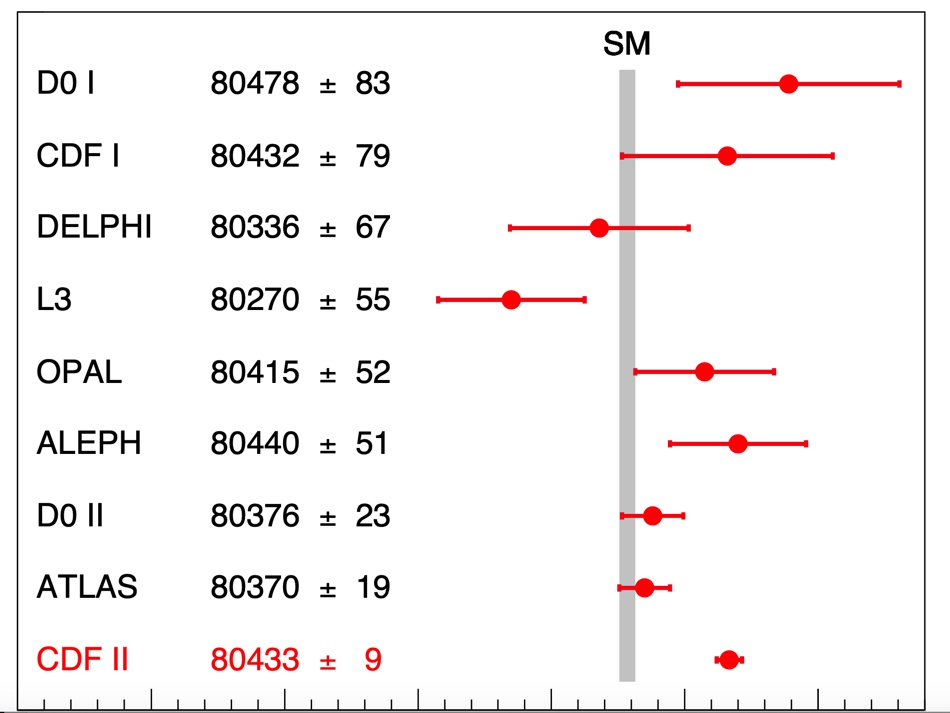
\includegraphics[height=10cm, width=12cm]{pictures/w-boson-comparisons.jpeg}
 \label{fig:1.4}
\end{figure}

利用费米实验室的Tevatron对撞机产生的高能粒子碰撞和对撞机探测器(CDF)收集的数据,研究人员收集了1985年至2011年间包含W玻色子的大量数据,它基于对 420 万个 W 玻色子候选者的观察,大约是2012年发布的合作分析中使用的数量的四倍。并且花了十年的时间来完成所有的细节和必要的检查,科学家们现在已经以 0.01\%的精度确定了粒子的质量(是之前最佳测量精度的两倍),得到了迄今为止精度最可靠的测量结果:$M_W=(80433.5\pm9.4)$MeV。(见上\textbf{图\ref{fig:1.4}})

通过合成以上两个数据的独立不确定度,我们可以得到测量值和标准模型预期值之间的差异存在$7\sigma$的偏差。这显示出了标准模型框架下,理论和实验的值产生了聚大冲突。如果无潜在错误,此测量表明可能需要改进标准模型计算或扩展模型。

科学界对这个结果也是众说纷纭——费米实验室副主任Joe Lykken指出:“虽然这是一个有趣的结果,但测量结果需要通过另一个实验来确认,然后才能完全解释。” 德克萨斯农工大学CDF联合发言人David Toback补充道:“如果实验值和预期值之间的差异是由于某种新的粒子或亚原子相互作用造成的,这是一种可能性,那么它很有可能在未来的实验中被发现。”

\section{LHC上的CMS实验}
\subsection{大型强子对撞机(LHC)}
大型强子对撞机(LHC)是世界上最大、能量最高的粒子对撞机。它由欧洲核研究组织(CERN)于1998年至2008年间与 10000多名科学家、数百所大学和实验室以及 100多个国家合作建造。它位于日内瓦附近法国-瑞士边界下方的一条周长27公里(17 英里)、深达175米(574英尺)的隧道中(如\textbf{图\ref{fig:1.5}}所示)。


LHC上的第一轮运行(RUN I)开始于2010年每个质子束3.5TeV的能量对撞,约为之前世界纪录的四倍。升级后,RUN II达到每质子束6.5TeV(总碰撞能量13TeV,目前世界最高)。2018年底停产三年,正在进一步升级到RUN III。

\begin{figure}[H]
 \centering
 \caption{LHC的探测器和部门分布\cite{LHC-complex}}
 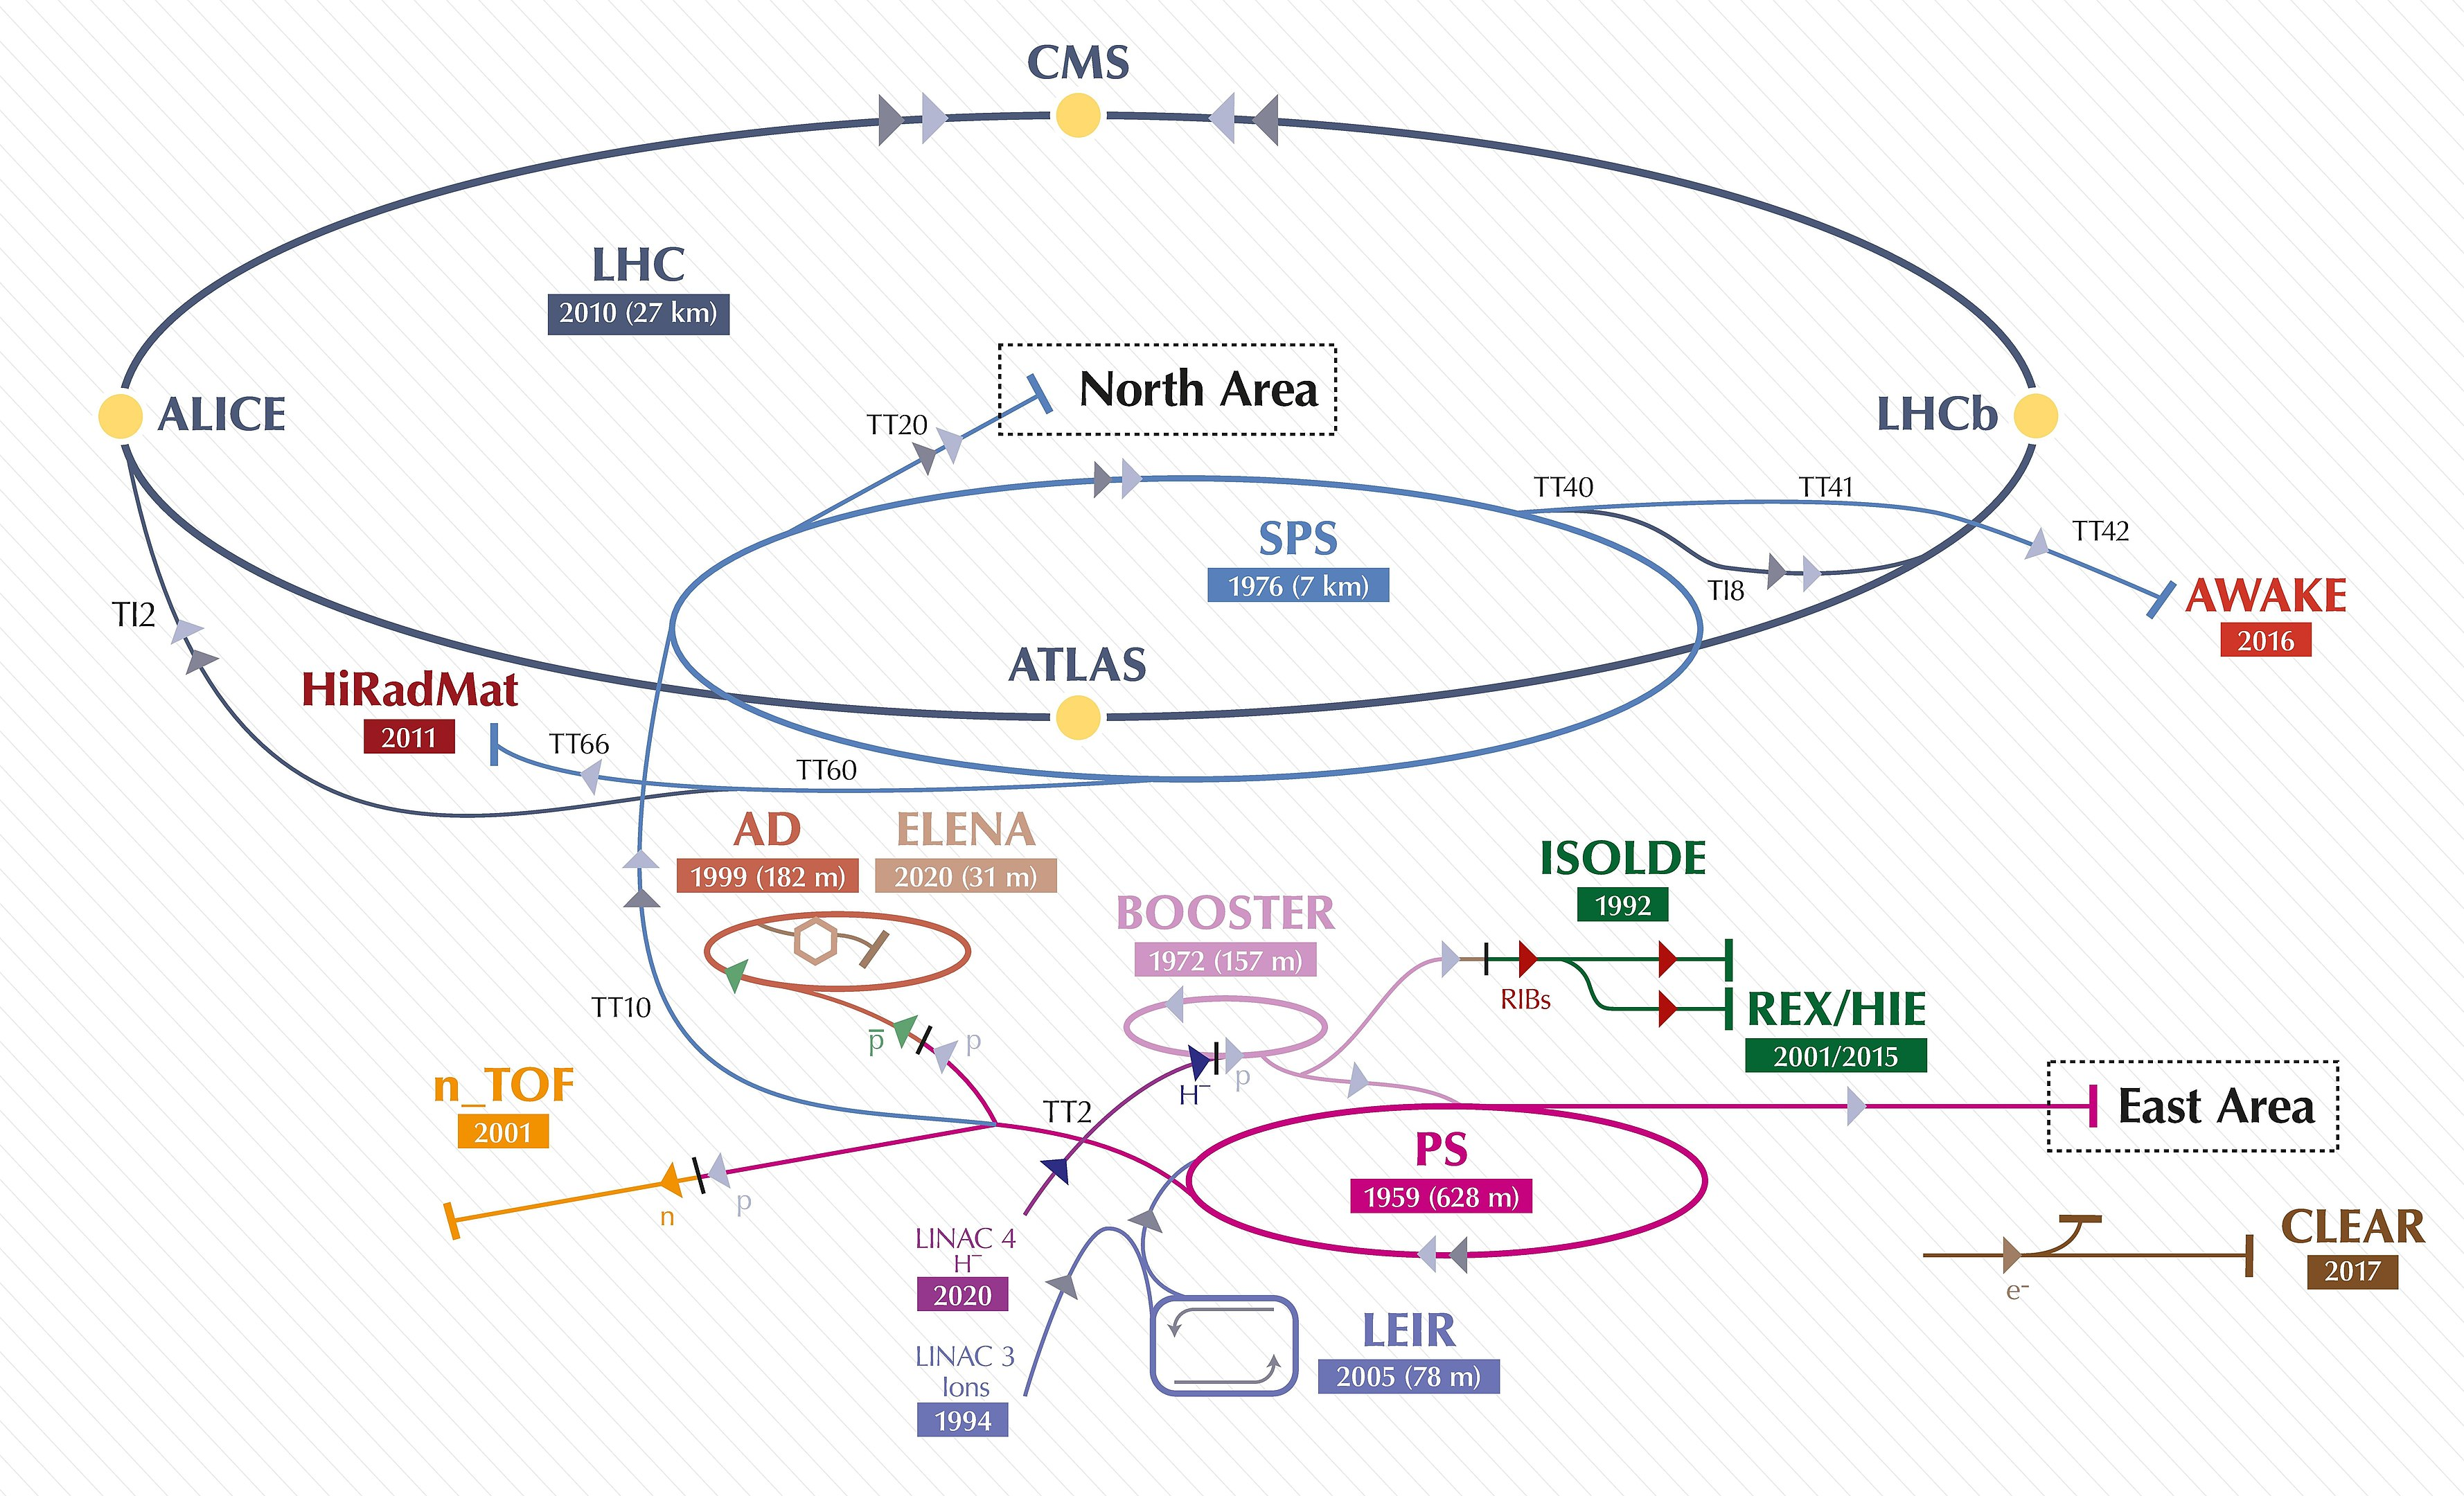
\includegraphics[height=8cm, width=14cm]{pictures/CERN_accelerator_complex_(cropped_2).jpeg}
 \label{fig:1.5}
\end{figure}


LHC上有四个交叉点,加速粒子在这些交叉点发生碰撞。LHC还有七个探测器,每个设用于检测不同的现象,位于交叉点周围。LHC主要碰撞质子束,但它也可以加速重离子束:铅-铅碰撞和质子-铅碰撞通常每年进行一个月。

LHC的目标是让物理学家能够测试不同粒子物理理论的预测,包括测量希格斯玻色子的性质,寻找超对称理论和其他未解决的粒子物理问题。

\subsection{紧凑缪子螺线管实验(CMS)}
紧凑型介子螺线管(CMS)实验是在瑞士和法国欧洲核子研究中心的大型强子对撞机(LHC) 上建造的两个大型通用粒子物理探测器之一。CMS实验的目标是研究广泛的物理学,包括寻找希格斯玻色子、额外维度和可能构成暗物质的粒子。

CMS探测器长21m,直径15m,重约14000吨。来自47个国家/地区的206个科研机构的4000 多人组成的CMS合作组建造并运行了探测器。2012年7月,CMS实验组与ATLAS实验组联合声明发现了希格斯玻色子。

CMS实验的主要目标是:
\begin{itemize}
    \item 在TeV尺度上探索物理学
    \item 进一步研究CMS和ATLAS已经发现的希格斯玻色子的性质
    \item 寻找超出标准模型的物理证据,例如超对称或额外维度
    \item 研究重离子碰撞的各个方面
\end{itemize}

位于LHC环另一侧的ATLAS实验的设计考虑了相似的目标,这两个实验旨在相互补充,以扩大范围并提供对研究结果的证实。CMS和ATLAS使用不同的技术解决方案和探测器磁铁系统设计来实现目标。

\begin{figure}[H]
 \centering
 \caption{CMS探测器剖面图\cite{cms-detector}}
 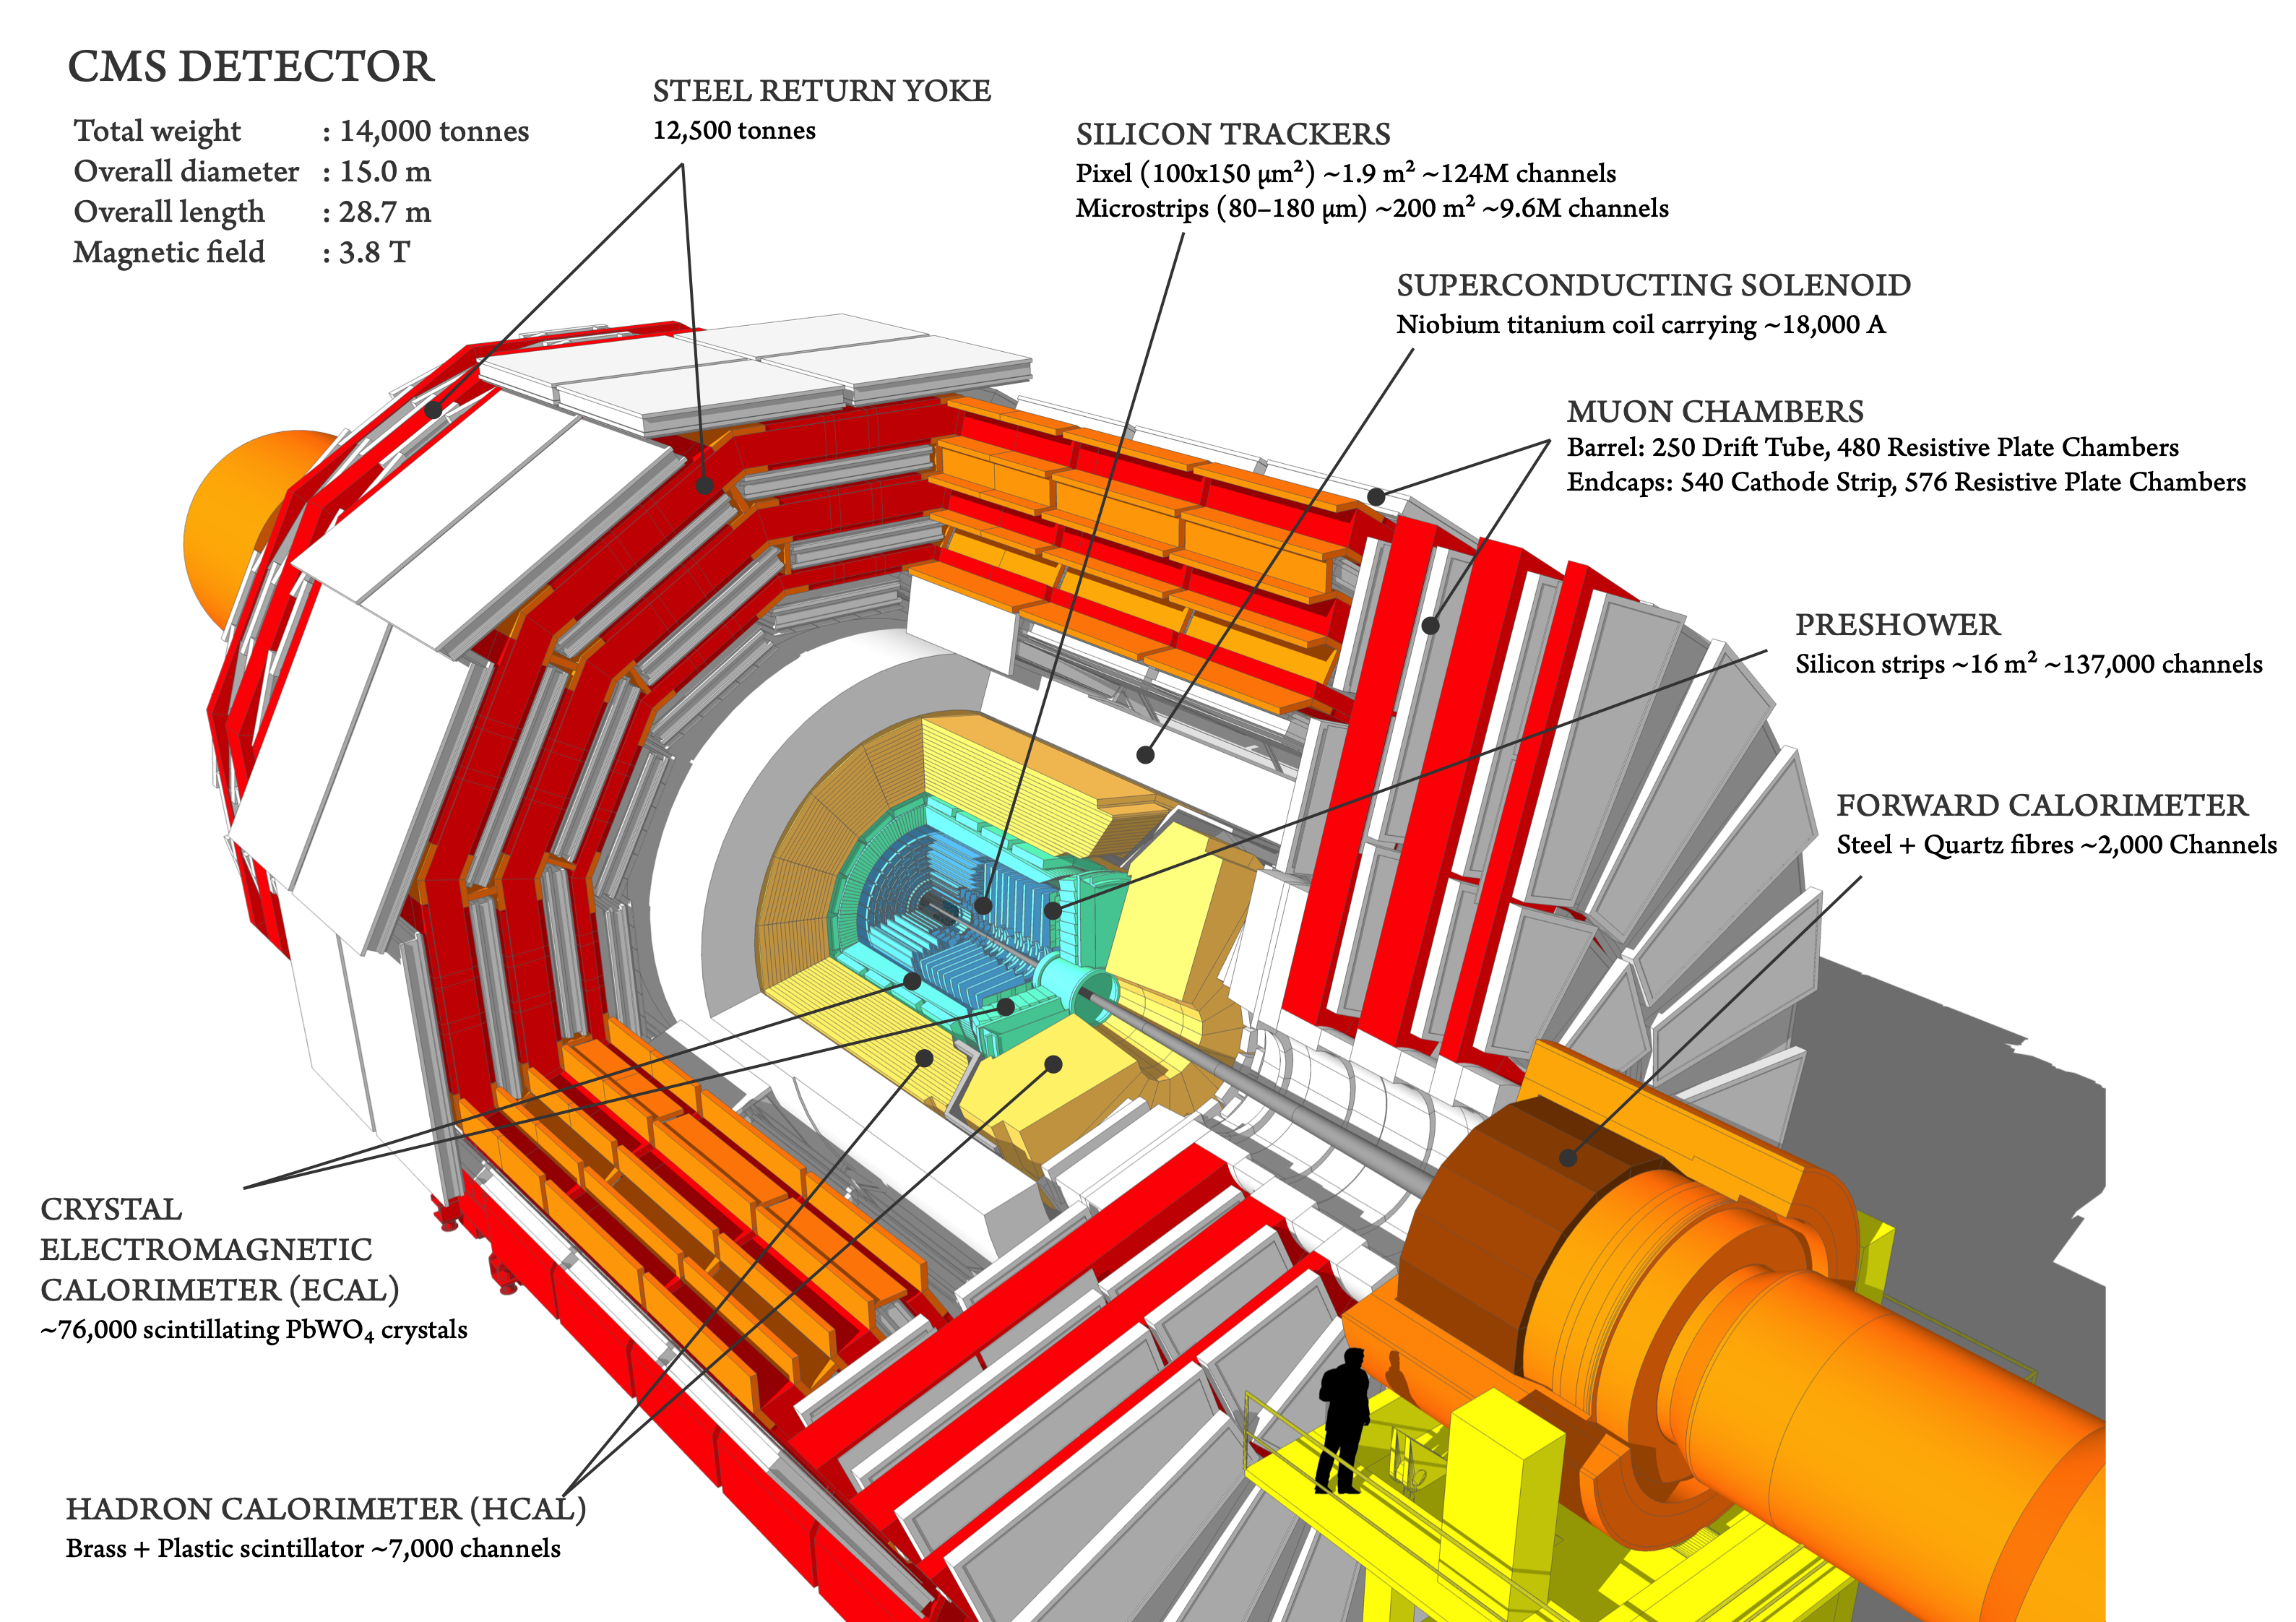
\includegraphics[height=9cm, width=13cm]{pictures/CMS_detector.png}
 \label{fig:1.6}
\end{figure}

CMS被设计为通用探测器,能够在LHC粒子加速器的质心能量0.9-13TeV下研究质子碰撞的许多物理内容。CMS探测器围绕一个巨大的螺线管磁铁构建。它采用圆柱形超导电缆线圈的形式,产生4T的磁场,大约是地球磁场的100000倍。磁场被限制产生在12500吨重量的的探测器主体——钢轭内(如\textbf{图\ref{fig:1.6}}所示)。CMS探测器的一个不同寻常的特点是,它不像大型强子对撞机实验中的其他巨型探测器那样在地下原位建造,而是在地面上建造,然后分15个部分被降到地下并重新组装。

CMS探测器包含用于测量光子、电子、$\mu$子和其他碰撞产物的能量和动量的子系统。最内层是硅基径迹探测器,被闪烁晶体电磁量能器所包裹,而闪烁晶体电磁量能器本身又被一个强子采样量能器包围。径迹探测器和量能器足够紧凑,可以安装在CMS螺线管内,该螺线管可产生3.8T的强大磁场。磁体外部是大型μ子探测器,它们位于磁铁的返回轭内。